\documentclass[12pt, english]{scrartcl} %Koma-Klasse "Artikel" mit 12pt Schrift
\usepackage[left=20mm, right=20mm, top= 25mm, bottom=25mm]{geometry}  % Seitenrändern
\usepackage{graphicx} %zum Einfügen von Bildern
\usepackage[english]{babel} %englische Silbentrennung
\usepackage{multicol}
\usepackage{graphicx}
\usepackage{caption}
\usepackage{textcomp}
\usepackage{lipsum}
\usepackage{gensymb}
\newenvironment{Figure}
  {\par\medskip\noindent\minipage{\linewidth}}
  {\endminipage\par\medskip}
\graphicspath{./graphics/}
\usepackage{siunitx}

\sisetup{separate-uncertainty}
\usepackage{braket}

\title{F18/38 Atmospheric Spectroscopy}
\author{Carsten L{\"u}th \and Michael Dorkenwald}
\date{\today}

\begin{document}
\maketitle

\begin{multicols}{2}


\section{Abstract}
In this experiment the trace gases Nitrogendioxid ($NO_2$) and Ozone ($O_3$) are examined with DOASIS. These gases play an important role for life on earth. Therefore it is important to have a method to determine the concentration in the air. The DOASIS (DOAS Intelligent System) was developed at the Institut for Environmental physics at University Heidelberg
\section{Introduction}
The atmosphere is the gas cover surrounding of an astronomic object due to its gravitation. The experiment on which this report is based analyses the atmosphere of the earth and how we humans influence it by the usage of fossil fuels.\\
The earth's atmosphere is divided into troposphere, stratosphere, mesosphere, thermosphere and exosphere. The UV-radiation of the sun is almost purely absorbed (roughly $95-99\%$) in the stratosphere by the gas ozone ($O_3$). 
Due to the emission of climate gases or radicals for catalytic ozone destruction such as $NO$ humans impacted the concentration of $O_3$ in stratosphere and troposphere.\\  
This lead to the creation of the Ozone-hole over antarctica (and the arctica) as well as health issues in urban or strongly industrialized areas due to photochemical smog.\\
The overarching goal of the experiments was to analyse the $O_3$ and $NO_2$ concentrations over the course of the day and their spatial arrangement.\\
All measurements in this experiment were done with the \textbf{D}ifferential \textbf{O}ptical \textbf{A}bsorption \textbf{S}pectroscopy method. 
First we conducted a mini experiment with a $NO_2$ gas-cell to learn the basis functions of our spectrometer and the methods used in combination to measure the \textbf{S}lant \textbf{C}olumn \textbf{D}ensity with an active source of light.\\
Second we did a Zenith sky measurement to determine the \textbf{V}ertical \textbf{C}olumn \textbf{D}ensity of $O_3$ and $NO_2$ over the course of a day. 
In the last measurement we used the principle of Multi-Axis-DOAS by measuring the SCD for different elevation angles the incoming light to determine the density of $O_3$ and $NO_2$ in the troposphere.\\
\section{Background}
In the following the most important principles to understand our measurements and conclusions are briefly introduced and a bit of reasoning for their importance.
\subsection{Ozone and Nitrogendioxid}
The $O_3$ concentration in the air is the result of an equilibrium for creation and destruction of $0_3$ molecules. Most of the $O_3$ from a VCD is located in the stratosphere because the $O_2$ photolysis is part of the reaction to create $O_3$. The probability a $O_2$ photolysis scales with the density of $O_2$ and requires a photon with a wavelength smaller then $242nm$ which mostly get absorbed by the photolysis happening in the stratosphere.\\
To predict the VCD of $O_3$ two theoretical models are used together. The Chapman Cycle describes the reactions between $O_2$, $O_3$ and photons. While the Catalytic ozone destruction describes how radicals of the groups $HO_X$ ($H, OH, HO_2$), $NO_X$ ($NO_2,NO$), $ClO_X$ ($Cl, ClO$) and $BrO_X$ ($Br,BrO$) greatly accelerate the ozone destruction. These radicals can cycle through thousands of iterations of the accelerated destruction cycle, while only being removed by chemical reactions or sedimentation.\\
$NO_2$ being one of those radicals is mainly a secondary pollutant, meaning that it is not a direct emission of burning fossil fuels. Instead it is mainly produced by a reaction between $NO$ and $O_3$. The most important mechanism for the formation of $NO$ is the Zel'Dovic cycle describing the \textit{thermal} formation of $NO$, the reaction between very high energetic $N_2$ and $O_2$.\\
The oxidation to $NO_2$ is explained by equations \ref{o3recomb} - \ref{photolysis} which result in the \textbf{photostationary state} between $O_3$ and $NO_X$.
\begin{equation}\label{o3recomb}
O + O_2 + M \rightarrow O_3 + M 
\end{equation}
\begin{equation}\label{steady}
O_3 + NO \Longleftrightarrow NO_2 +O_2
\end{equation}
\begin{equation}\label{photolysis}
NO_2 + h\nu(\lambda < 410 nm) \rightarrow NO + O
\end{equation}
The molecule or atom $M$ is only needed for the conservation of momentum.
The steady state resulting from the photostationary state can be described by the \textbf{Leighton ratio} (eq. \ref{Leighton}).
\begin{equation}\label{Leighton}
\frac{[NO]}{[NO_2]} = \frac{j_{NO_2}}{k_{O_3+NO} \cdot [O_3] }
\end{equation}
The photolysis rate, depending on sun angle and intensity, is described by $j_{NO_2}$ and  $k_{O_3+NO}$ is the reaction constant in equation \ref{steady}.\\
\paragraph{Diurnal Cycle}
During a day the $NO_2$ and $NO$ concentrations change cyclically due to the building of $NO_3$ and $NO_5$. In the \textit{morning} the mixing ratio of $NO_2$ in the stratosphere increases due to the dissociation of $NO_5$ excited by photons. During the \textit{day} $NO$, $NO_2$ and $O_3$ are in a photostationary balance and in the \textit{evening} the photolysis (eq. \ref{photolysis}) decreases and $NO$ is no longer created, leading to an increase of $NO_2$. At \textit{night} $NO_2$ forms $NO_5$ again.
\paragraph{Photochemical smog}
Photochemical smog occurs when high levels of volaticle organic compounds (VOCs) and $NO_X$ are emitted into thermal inversion layer so that are trapped closely to the ground. This leads to very high ozone levels in the troposphere because in the presence of VOCs there is another reaction path for the conversion of $NO$ to $NO_2$. The reaction between VOCs and $NO_X$ means that the Leighton ratio is no longer valid with the photostationary balance and destruction of $O_3$. 
 \subsection{The DOAS Measurement System}
The DOAS measurement system is used for detection of trace gases in the atmosphere. It's principle is to measure the absorption spectrum of specific substances using the \textit{Lambert Beer} law for $n$ different absorbers (eq. \ref{beer}).
\begin{equation}\label{beer}
I(\lambda, L) = I_0(\lambda) \cdot \exp (- \int^{L(\lambda)}_0 \sum_i^n \sigma_i(\lambda) \cdot \rho_i(s) ds)
\end{equation}
The absorption cross section is defined as $\sigma$ and the SCD is defined (in eq. \ref{SCD}) as the integrated concentration $\rho$ of a trace gas $i$ along the light path of length $L$.
\begin{equation}\label{SCD}
\text{SCD} = S_i(\lambda) =\int^{L(\lambda)}_0  \rho_i(s) ds)
\end{equation}
Because it is not possible to single out every different absorber to get a direct absorption spectrum for measurements in the atmosphere the DOAS method uses the fact that may processes in radiative transfer show broad or even smooth spectral characteristics. This stands in contrast to the narrowband absorption structures many trace gases exhibit. So the key concept of DOAS is the separation of spectral structures in narrowband and broadband components, called \textit{differential spectra}. With this method narrowband absorptions of trace gases can be detected.\\
When taking a DOAS measurement to to quantify the SCD of a specific trace gas in the atmosphere the \textit{Frauenhofer refence spectrum} $I_0$ because of the sun's structured spectrum. The Ring effect is the narrowing of absorption bands due to Raman scattering which also needs to be taken into account.\\
The light's broadband spectrum is mostly affected by Mie and Rayleigh scattering also some of the trace gases exhibit broad band absorption too. In the DOAS fit minimizing the quadratic deviation of the optical density $\tau$ (eq. \ref{tau}).
\begin{equation}\label{tau}
\tau = \log (\frac{I(\lambda)}{I_0(\lambda) }) = -R -\sum_i \sigma_i S_i - \sum_k b_k \lambda^k
\end{equation}
The broadband absorption is described by the polynomial $\sum_k b_k \lambda^k$ while the rest of the formula describes the narrowband features and $R$ is the Ring spectrum. The fit parameters are $S_i$ and the polynomial coefficients $b_k$ for a minimized residual.\\
The DOAS method can only detect a trace gas with an optical density larger than the residual.
\section{Meassurements}
In the following sections the conduction of our measurements is described. The spectrograph-detector used for the measurements is the Ocean Optics USB2000 based on the Czerny-Truner design and is located in a cooled housing unit. 
The telescopes are connected via a $400 \mu m$ diameter quarty fiber bundle (NA $0.22$) with the spectrometer. The spectrometer either can be connected to a telescope for atmospheric measurements or a lab telescope. \\
The initial few measurements were only used to compute the Background noise of the spectrometer, which consists of the electronic offset, dark current and the uncertainty of the light counts due to the under lying poisson distribution. After that the pixel to wavelength ratio of the spectrometer was calibrated with a mercury lamp using a polynomial fit. These measurements will note be further discussed.\\
\subsection{Nitrogendioxid gas-cell}
In this part of the experiment we measured the absorption of a $NO_2$ gas-cell in the spectrum of an Hg-lamp. Due to the nature of this measurement we could simplify the problem by using the fact that we have access to $I_0$ by taking a spectrum without the gas cell in the light path and then take a measurement with the gas-cell in the light path to measure $I$.\\
The integration time $t$ is $100ms$ and number of scans is equal to $100$. for both the measurement of $I$ and $I_0$
\subsection{Zenith sky measurements of a daycycle}
In this experiment we chose the zenith sky measurement spectra recorded on the daycycle of a sunny day. For zenith sky measurements the telescope is orientated straight up with an elevation angle ($\alpha$) of $90 \degree $. This can be seen in figure \ref{sza}.\\
\begin{Figure}
 \centering
 \captionsetup{format=plain}
 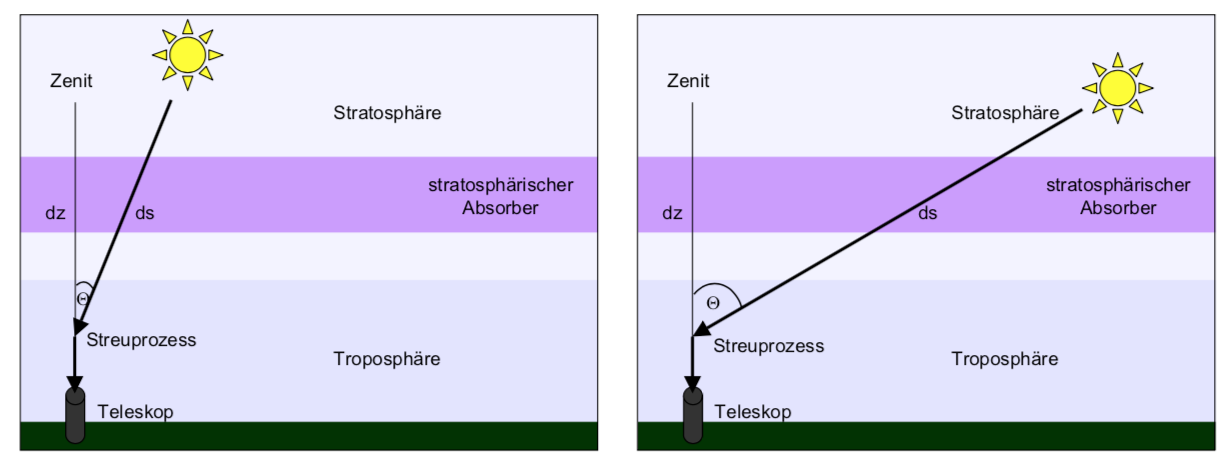
\includegraphics[width=\linewidth]{graphics/sza.png}
 \captionof{figure}{Light paths trough the atmosphere for a small (left) and high (right) SZA. The light path through the stratosphere is enhanced for higher SZA.}
 \label{sza}
\end{Figure}
We used the measurement with a minimal solar zenith angle ($\theta$) as Frauenhofer reference spectrum because it has the least interaction with the atmosphere due to the minimal path length. 
\subsection{Multi-Axis-DOAS}
In this part we measured spectra for different elevation angles ($\alpha$) of the telescope. For smaller elevation angles light entering the telescope is strongly scattered and has a longer path in the troposphere leading to an increased interaction with the gases found in the troposphere. This schematic can be seen in figure \ref{multiaxis}.
\begin{Figure}
 \centering
 \captionsetup{format=plain}
 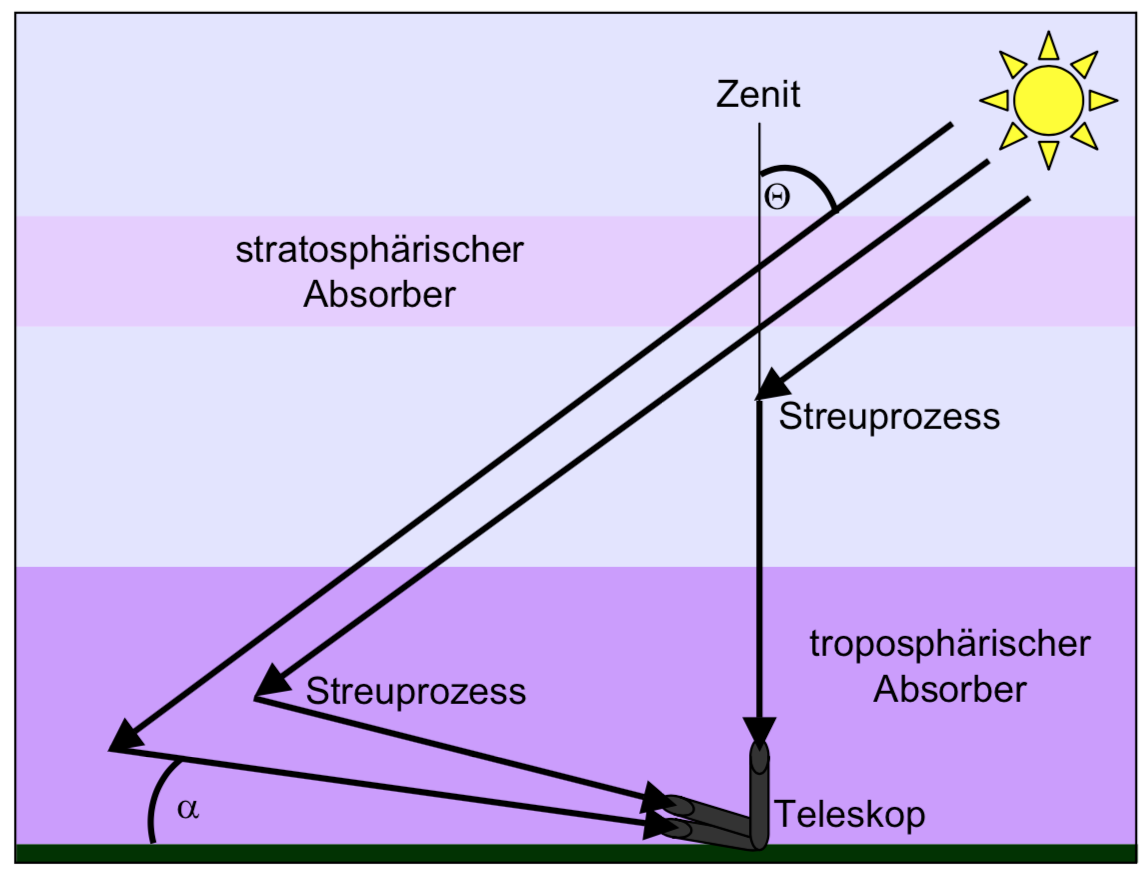
\includegraphics[width=\linewidth]{graphics/multiaxis.png}
 \captionof{figure}{Light paths for different elevation angles of the telescope at with identical SZA.}
 \label{multiaxis}
\end{Figure}
To measure the trace gas concentration in the troposphere it is important that the measurements for the different elevation angles of the telescope have a very similar SZA. This means that they should be taken in the shortest frame of time in successive order possible.\\
The Frauenhofer reference spectrum for these measurements was taken with $\alpha = 90\deg$ to minimize the path length in the troposphere and two measurements with $\alpha$ being $7 \deg$ and $9 \deg$.\\
These measurements were taken 4 times on the 5th December 2018. The weather was a bit cloudy but mostly clear with a weak sun intensity.
The integration time of $600$ms lead to a sufficient saturation and 600 scans were used as parameters.
\section{Results}
First of all, we computed the offset and the dark current and corrected every measurements with these values. Moreover, we calibrated the spectrometer with the mercuray spectra. 
\subsection{Nitrogendioxid gas-cell}
First we adapted the high resolution wavelength reference measurements to our spectrometer used in this experiment. This is done by convolving the high resolution reference cross-section with the DOAS slit function. We used the Lambert-Beer law and performed a least-squares fit to obtain the concentration of the gas-cell:
\begin{equation}
\chi^2 = [\log(\frac{I(\lambda)}{I_0(\lambda)})- \sigma_{NO_2} \cdot S_{NO2} - \sum_k b_k \lambda^k ]^2
\end{equation}
From the fit we obtained the optimal value for $S_{NO2}= \rho \cdot L$. This was then used to compute the density:
\begin{equation}
\rho = (2.81 \pm 0.07 ) \cdot 10^{-7} \frac{\text{mol}}{\text{cm}^3}
\end{equation}
and the mixture ratio:
\begin{equation}
r_{mix} = (6.29 \pm 0.39) \cdot 10^3 \text{ppm}
\end{equation}
\subsection{Zenith sky measurements of a daycycle}
We picked a sunny day for our evaluation with the frauenhofer reference number: T00562103 and the spectrum reference number: T0056227. We used a high solar zenith angle because the approximation for the air mass factor (AMF) is only valid for $\theta \geq 76 \degree$. First, we evaluate the approach on a single measurement by means we optmized the fit setting. For $NO_2$ we used the fit range: $[426-449] nm$ and for $O_3$: $[327-339] nm$. Afterwards, we evaluated the other spectras for that day.
We obtained with DOAS least squares fit the SCD values for different traces gases, namely ozone and nitrogendioxid. Those values were then plotted as a function of time of day and can be seen in figures \ref{NO2} and \ref{O2}.
\begin{Figure}
 \centering
 \captionsetup{format=plain}
 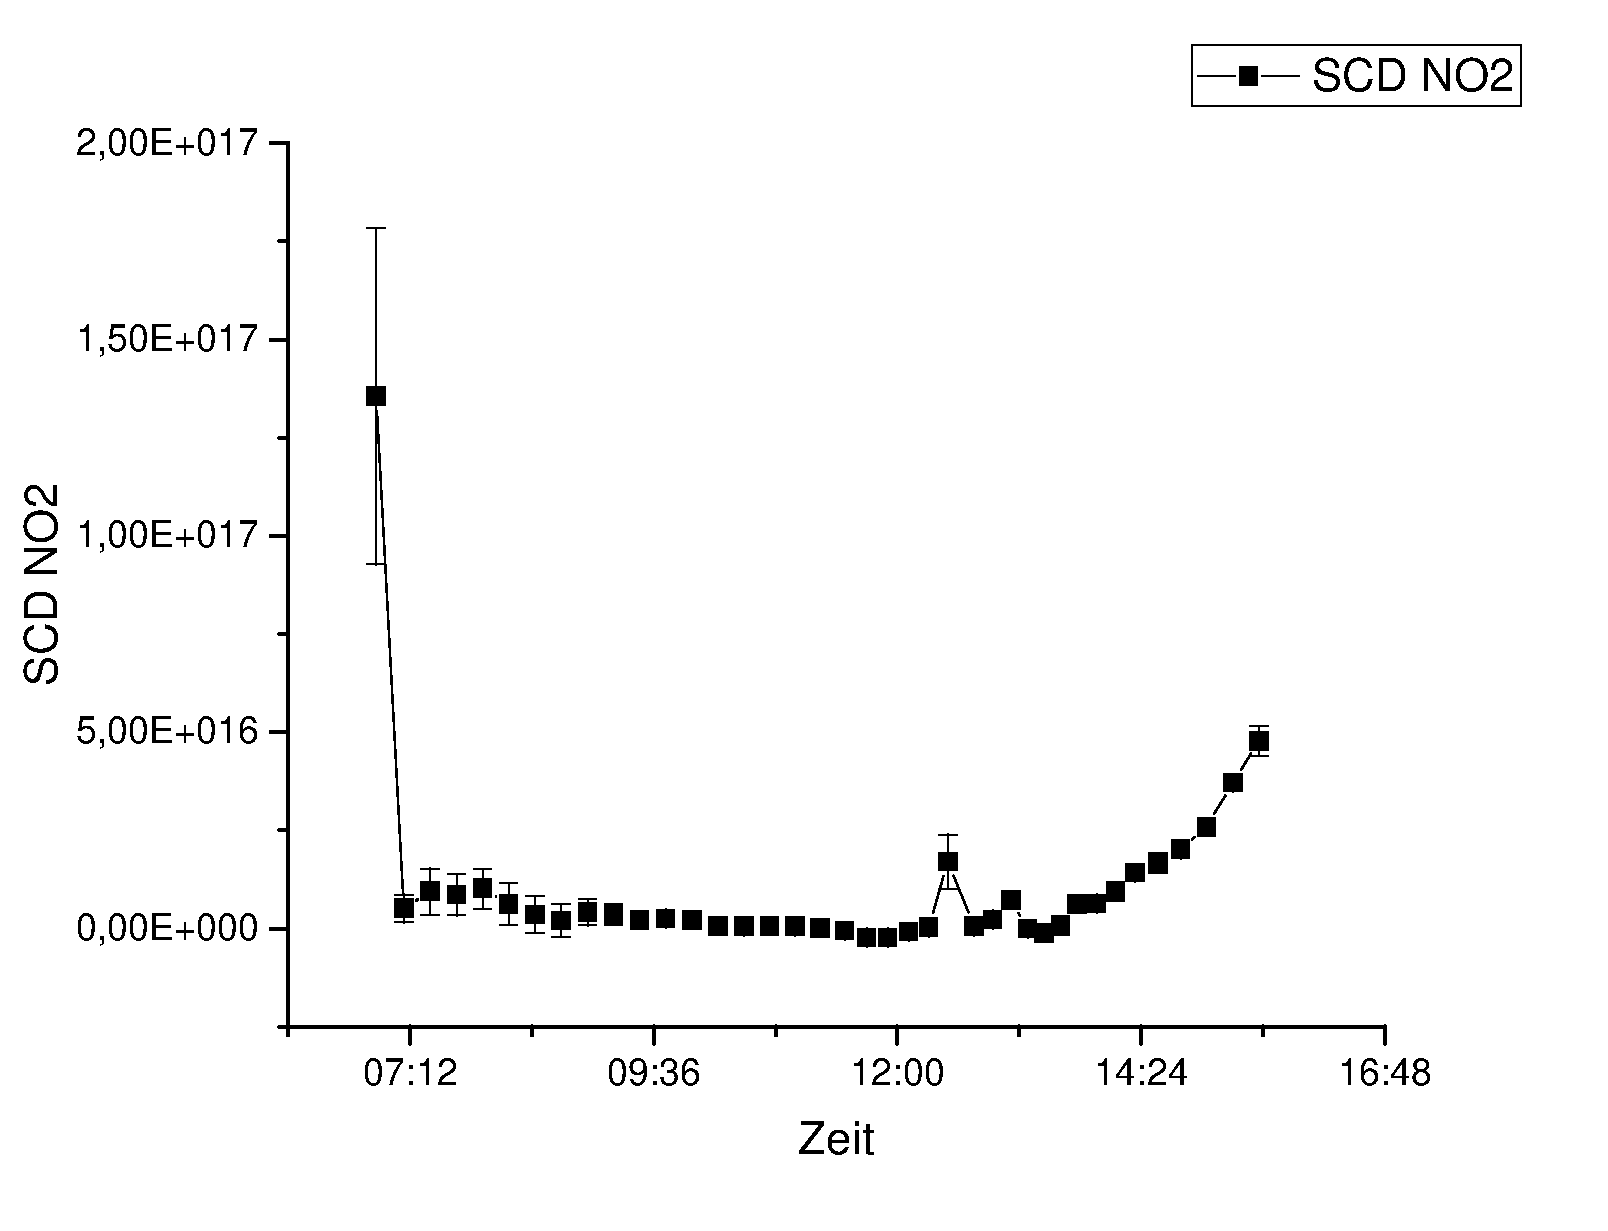
\includegraphics[width=\linewidth]{graphics/SCDNO2.pdf}
 \captionof{figure}{$\Delta$ SCD for $NO_2$ as a function of time of day}
 \label{NO2}
\end{Figure}
\begin{Figure}
 \centering
 \captionsetup{format=plain}
 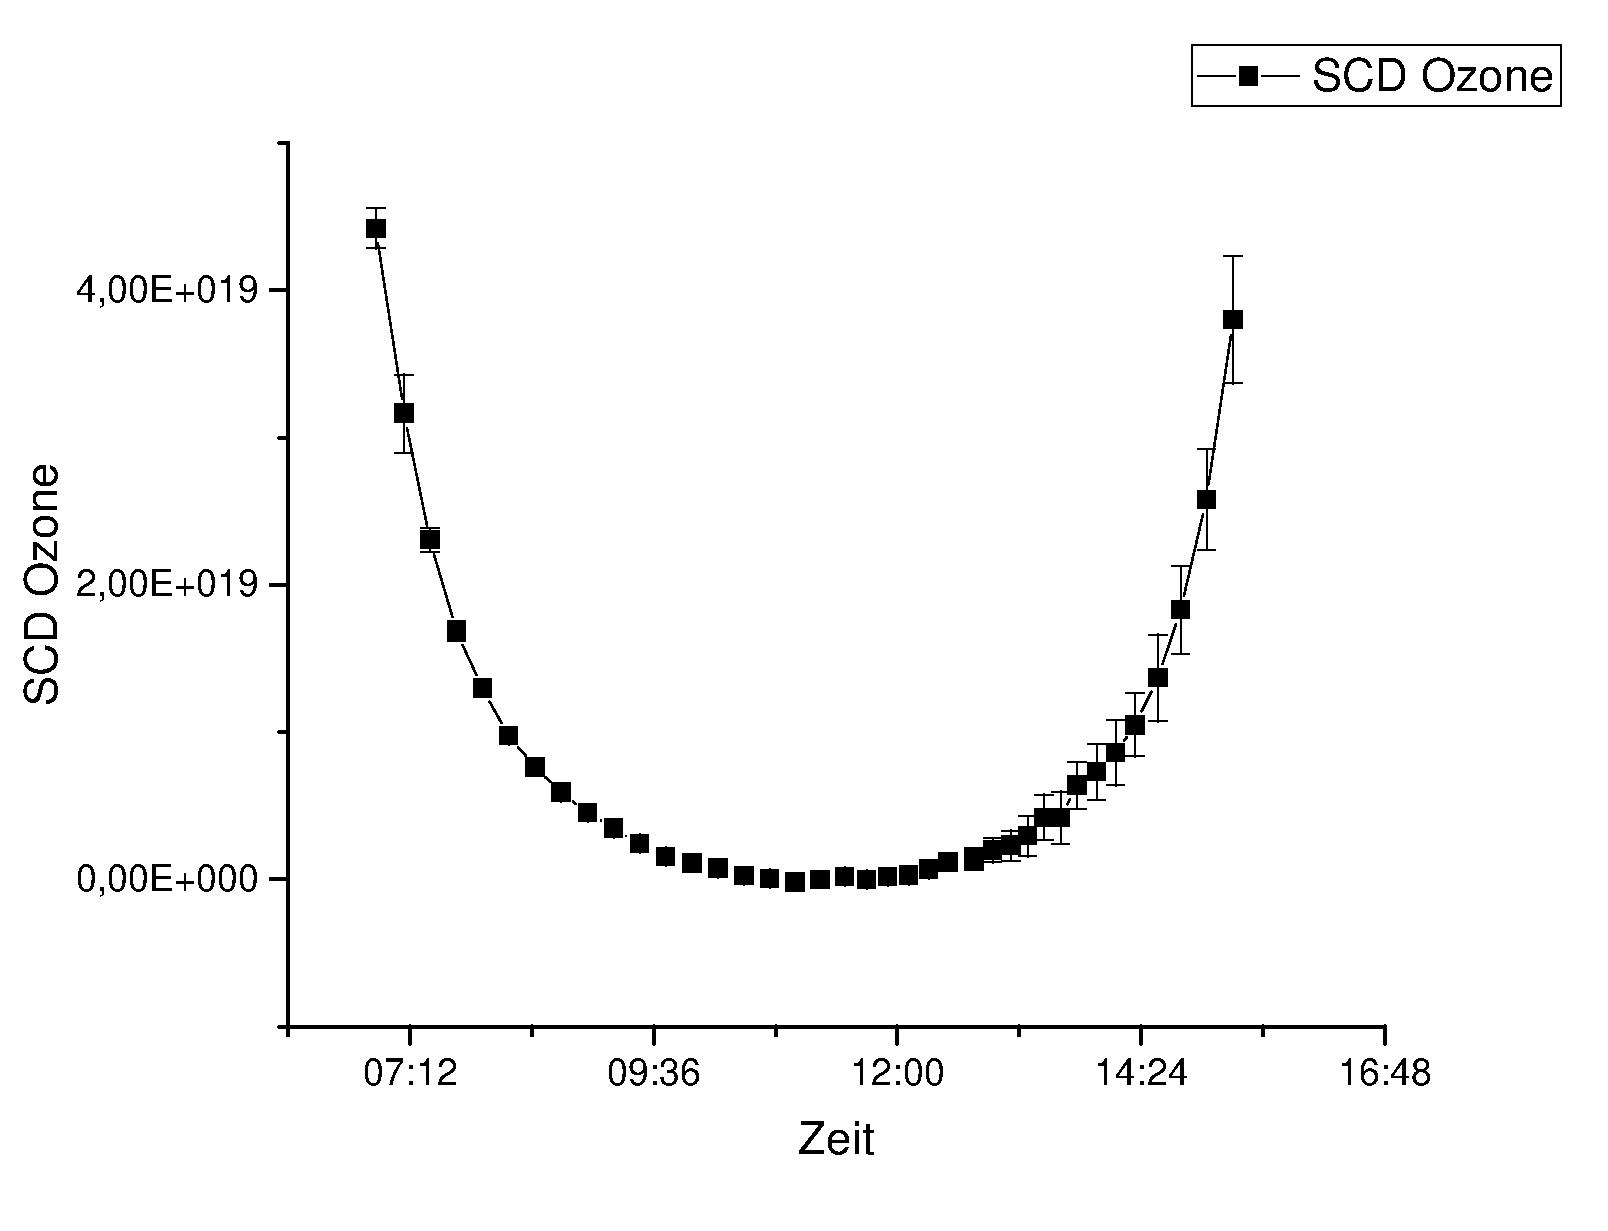
\includegraphics[width=\linewidth]{graphics/SCDOzone2.pdf}
 \captionof{figure}{$\Delta$ SCD for $O_3$ as a function of time of day}
  \label{O2}
\end{Figure}
\begin{Figure}
 \centering
 \captionsetup{format=plain}
 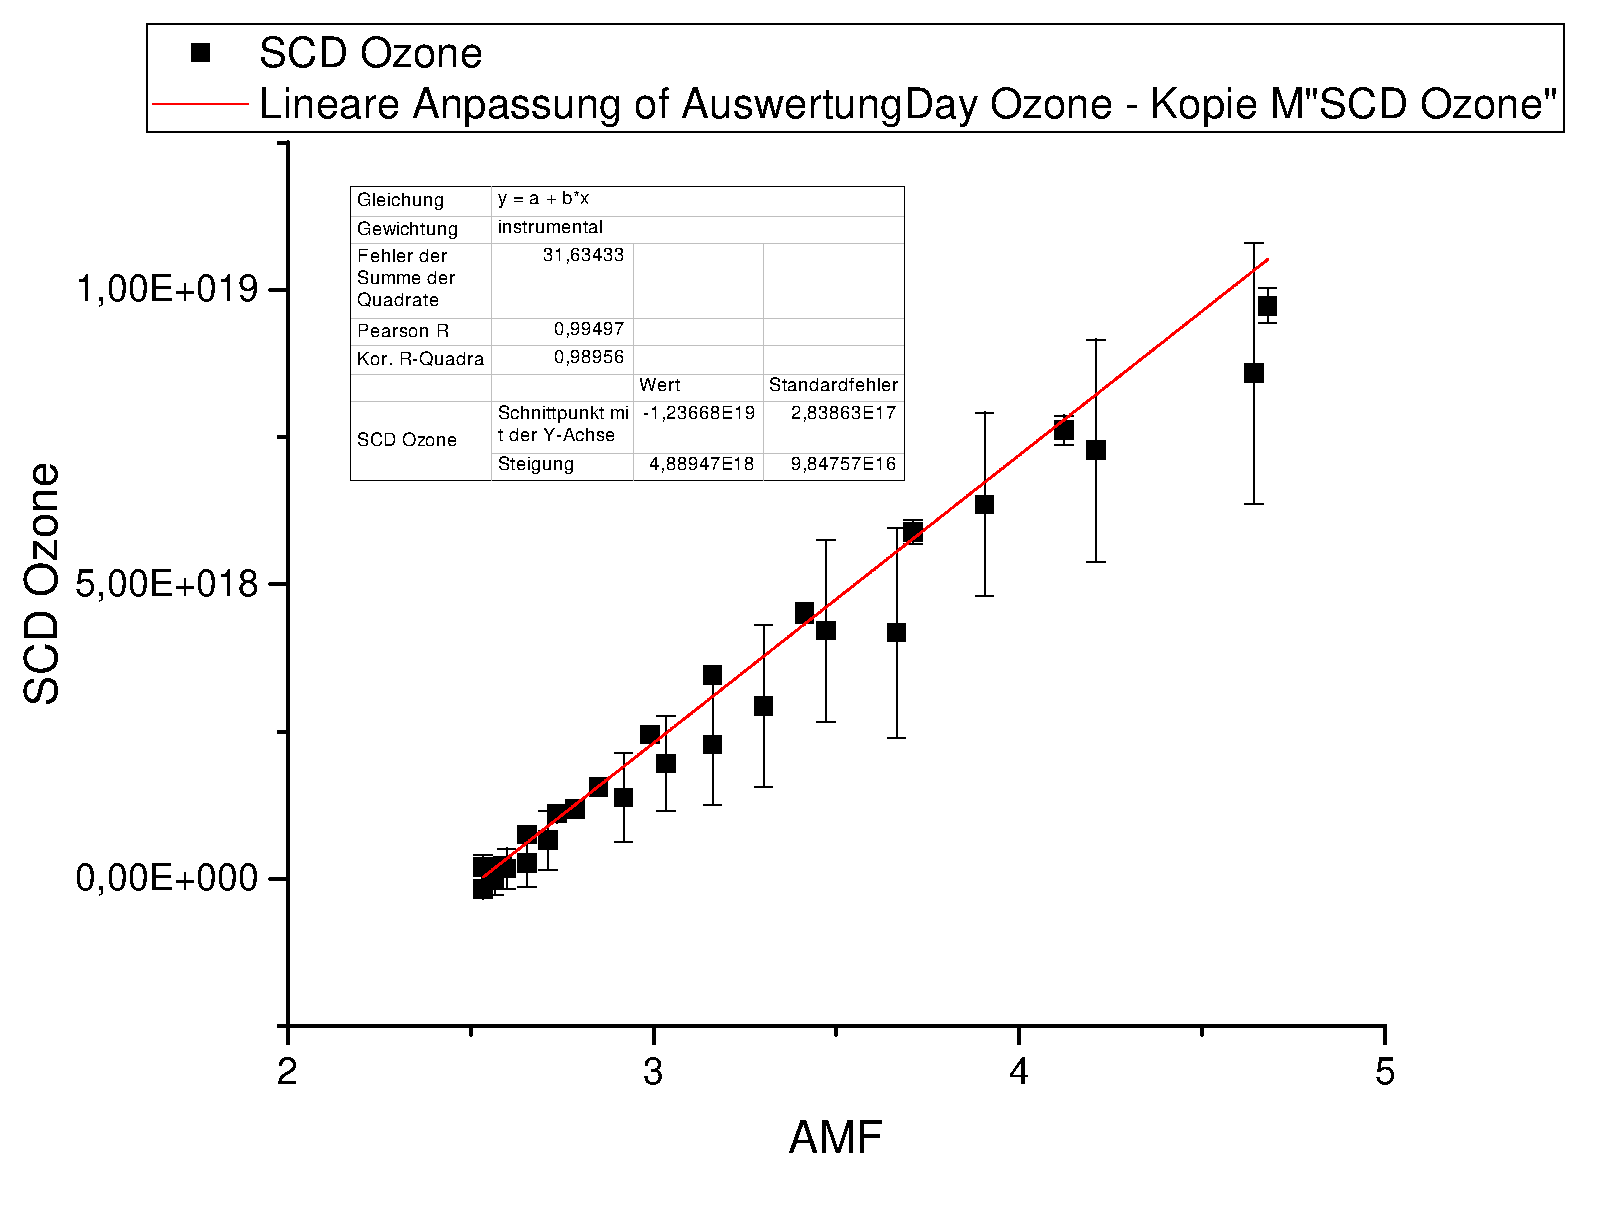
\includegraphics[width=\linewidth]{graphics/o3langley.pdf}
 \captionof{figure}{Langley Plot for the ozone measurement}
  \label{Lang}
\end{Figure}
\begin{Figure}
 \centering
 \captionsetup{format=plain}
 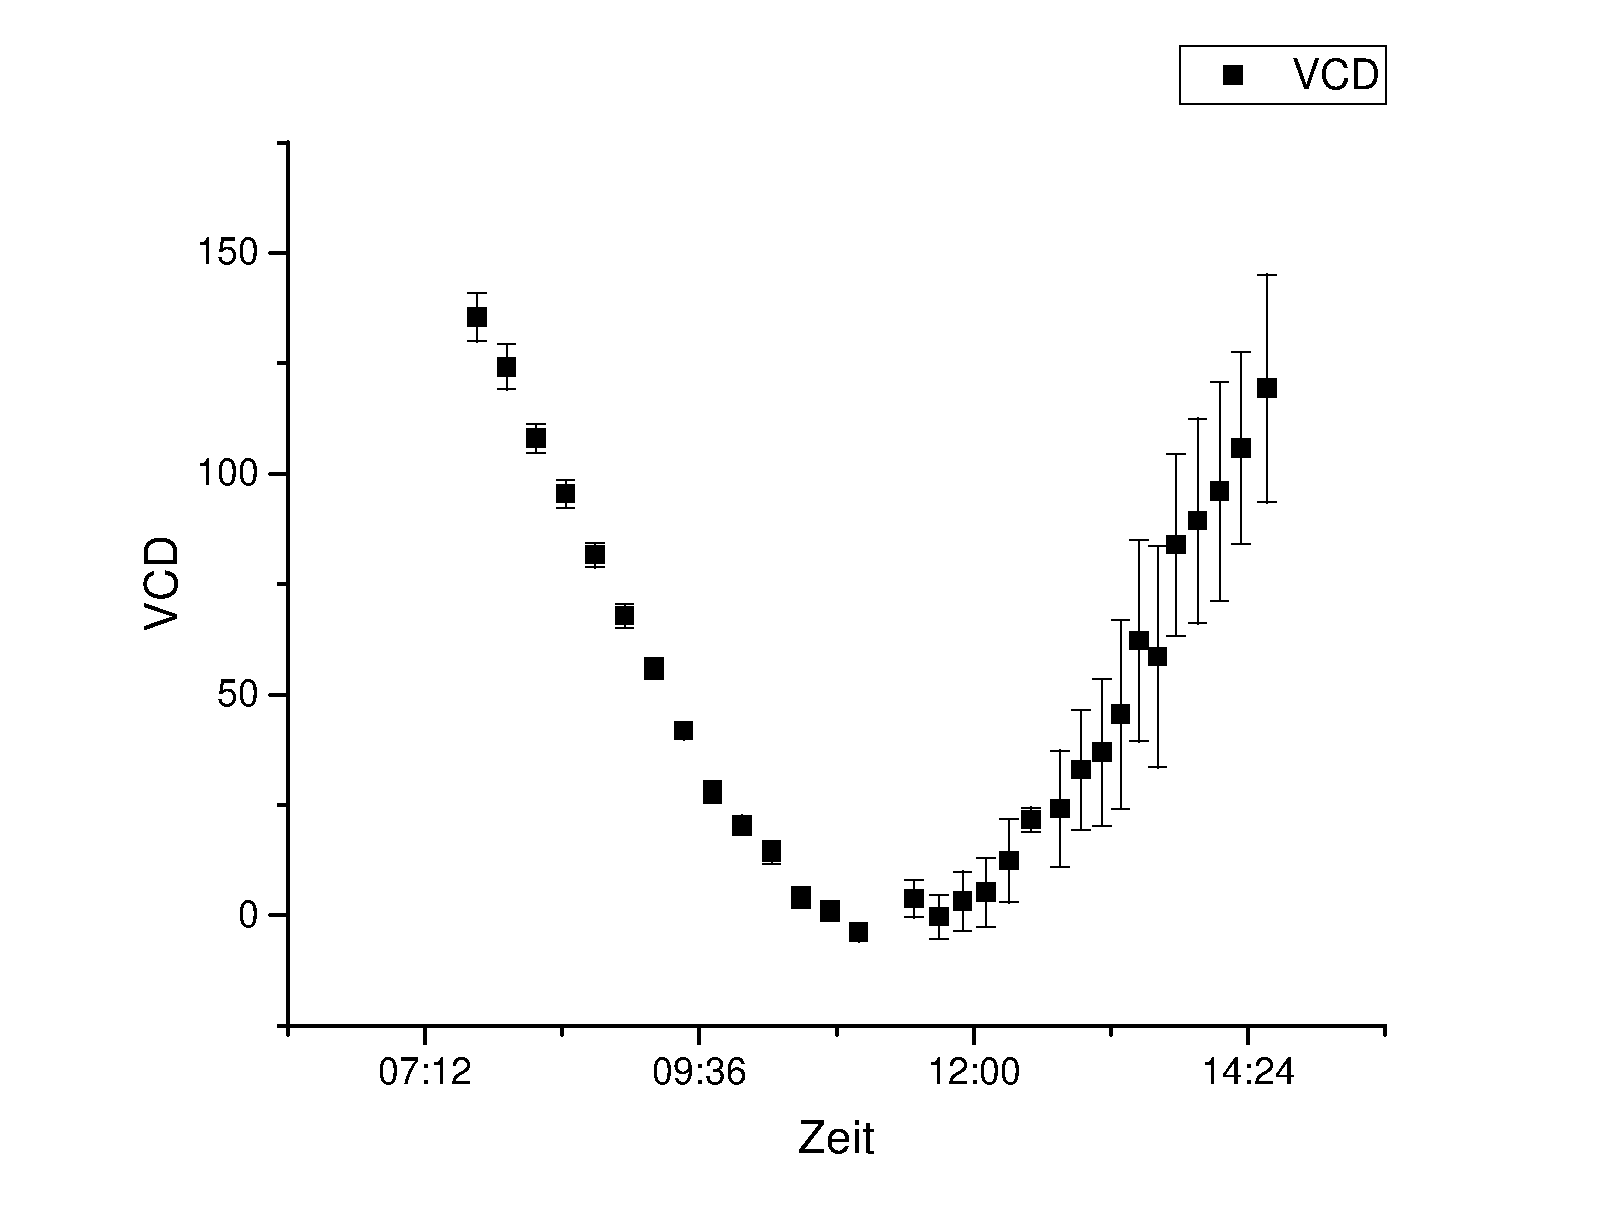
\includegraphics[width=\linewidth]{graphics/03vcd.pdf}
 \captionof{figure}{VCD as a function of time}
  \label{vcd}
\end{Figure}
In figure \ref{vcd} the vertical column density is plotted against time. The VCD can be computed with $VCD = SCD \cdot AMF$ provides the most useful and directly interpretable information on the distribution and concentration of trace gases. AMF can be approximated by: $AMF \approx \frac{1}{cos(\theta)}$. The U-shape of the $NO_2$ profile is caused by stratospheric $NO_2$. The U-shape of ozone is caused by cosmic radiation and can be confirmed by theory. In figure \ref{Lang} the $\Delta$ SCD is plotted against the AMF factor and we performed a linear fit for AMF $\leq 3.5$. With the extrapolation we obtained the slant column density in the Fraunhoer reference $SCD_{ref} =( 4.89\pm 0.10 ) \cdot 10^{18} $.
\subsection{Multi-Axis-DOAS}
Here we want to gain insight into the verticla distribution of trace gases ($NO_2$ and $O_4$)in the atmosphere. To this extent, scattered light spectra are recorded using differnt ($7 \degree, 12 \degree \text{\ and\ } 90 \degree$) telescope elevation angles. The $90 \degree$ measurement was used as a Fraunhofer reference spectrum for each set. In figure \ref{angle} the SCD for $7 \degree \text{\ and\ } 12 \degree$ are plotted. We carried out 4 measurements for each angle and took the mean and for the error the standard deviation for each angle. 
\begin{Figure}
 \centering
 \captionsetup{format=plain}
 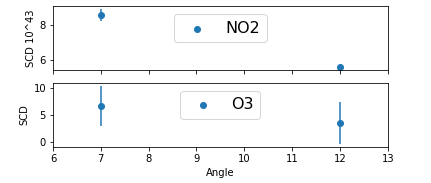
\includegraphics[width=\linewidth]{graphics/anglescd2.png}
 \captionof{figure}{$\Delta$ SCD as a function of the telescope elevation angle for ozone, $NO_2$ and $O_3$}
  \label{angle}
\end{Figure}
The SCD for $O_3$ and Ozone keeps constant by changing the angle. However, $NO_2$ decreases significantly by enlarging the elevation angle.
\section{Discussion}
The $\Delta$ SCD plot for ozone resembles the theoretical values well which can be seen in the good linear fit of the langley plot of the ozone $\Delta SCD$ against the AMF. 
From the elevation angle part it is clear that $NO_2$ is located in the stratosphere because of the significant change of SCD (scattering). Ozone and $O_4$ remain constant which means they are located in the troposphere. 
\end{multicols}

\end{document}